\chapter{\scshape Static background schemes}
\label{chapter:cvmix_background}


\minitoc
\vspace{.5cm}

\begin{mdframed}[backgroundcolor=lightgray!50]
This chapter presents options in CVMix code for prescribing static
(time independent) background diffusivities and viscosities.  The
following CVMix Fortran module is directly connected to the material
in this chapter:
\begin{align*} 
 &{\tt cvmix\_background.F90}
\end{align*}
\end{mdframed}

\section{Options for static background mixing coefficients}
\label{section:background-diffusivities}

\cite{Jochum2009} describes the large sensitivities found in climate
model simulations to the choice of background vertical diffusivities.
There are various options in CVMix code for specifying a static
background diffusivity and viscosity.  These mixing coefficients are
generally a function of space but remain the same value throughout the
simulation, and so are independent of the flow state.  These static
values are primarily determined for tracer diffusivity, with a Prandtl
number (ratio of diffusivity to viscosity) used to determine the
background viscosity.  A common choice for Prandtl number is 10,
although for some background diffusivities there is no corresponding
background viscosity (i.e., zero Prandtl number).


\section{The profile from Bryan-Lewis (1979)} 
\label{section:bryan-lewis}

A classic choice for background diffusivity is that proposed by
\cite{BryanLewis1979}, which has an arctangent form with smaller
values in the upper ocean and larger values beneath a pivot depth,
originally set to 1500~m
\begin{equation}
 \kappa_{\mbox{\tiny Bryan-Lewis}} = {\tt vdc1}
   + {\tt vdc2}  \;  \arctan\left[ ( |z| - {\tt dpth}) \,   {\tt linv}  \, \right].
\label{eq:bryan-lewis-function-pop}
\end{equation}
This is the form appearing in POP, where the parameters are defined as
follows.
\begin{itemize}

\item {\tt vdc1} is the diffusivity (squared length per time) at $|z|
  = {\tt dpth}$,

\item {\tt vdc2} = amplitude of variation for the diffusivity
  (squared length per time)

\item {\tt linv} is an inverse length scale 

\item {\tt dpth} is the vertical depth where the diffusivity equals
  {\tt vdc1}.

\end{itemize}
All lengths and diffusivities should be in MKS units.  In many
implementations, such as for GFDL-CM2.1, there is no corresponding
Bryan-Lewis viscosity, so the corresponding Bryan-Lewis Prandtl number
is zero.  But more generally, the viscosity is computed according to a
chosen Prandtl number.

In MOM5 and earlier versions of MOM, the form
(\ref{eq:bryan-lewis-function-pop}) is written in the somewhat more
cumbersome manner for historical reasons
\begin{equation}
 \kappa_{\mbox{\tiny Bryan-Lewis}} = {\tt convert} \left( 
       \,{\tt afkph}
   +  ({\tt dfkph}/\pi)  \; \arctan\left[ {\tt sfkph} (100 \,  |z| - {\tt zfkph} ) \right]
    \right),
\label{eq:bryan-lewis-function-mom}
\end{equation}
where {\tt afkph}, {\tt dfkph}, {\tt sfkph}, and {\tt zfkph} are
tunable constants, and ${\tt convert} = 1 \, \times
10^{-4}~\mbox{m}^{2}\mbox{s}^{-1}$ converts from the original CGS to
MKS.  The mapping between the MOM and POP forms
(\ref{eq:bryan-lewis-function-pop}) is given by the following
\begin{align}
{\tt vdc1} &= \kappa_{o} \, {\tt afkph}
\\
 {\tt vdc2} &= \kappa_{o} \, {\tt dfkph}/\pi
\\
 {\tt linv}     &= 100 \, {\tt sfkph}
\\
 {\tt dpth} &= 100 \, {\tt zfkph}.
\end{align}
We provide this mapping since Figure \ref{fig:bryan_lewis-profiles}
was constructed using the original MOM-based form.  Shown are two
examples of vertical diffusivity profiles used in the GFDL-CM2.1
simulations \citep[see][for discussion]{OMDT2005a}, with the values
given by 
\begin{align}
{\tt afkph} &=0.75
 \\
{\tt dfkph} &=0.95
\\
{\tt sfkph} &=4.5 \, \times 10^{-5}
\\
{\tt zfkph} &=2500
\label{fig:bryan_lewis-profiles-polar}
\end{align}
and for the equatorial region they are 
\begin{align}
{\tt afkph} &=0.65
\\
 {\tt dfkph} &=1.15
\\
 {\tt sfkph} &= 4.5 \, \times 10^{-5}
\\
 {\tt zfkph} &=2500.
\label{fig:bryan_lewis-profiles-tropics}
\end{align}



%%%%%%%%%%%%%%%%%%%% %%%%%%%%%%%%%%%%%%%%%%%%%
\begin{figure}[h!t]
\rule{\textwidth}{0.005in}
\begin{center}
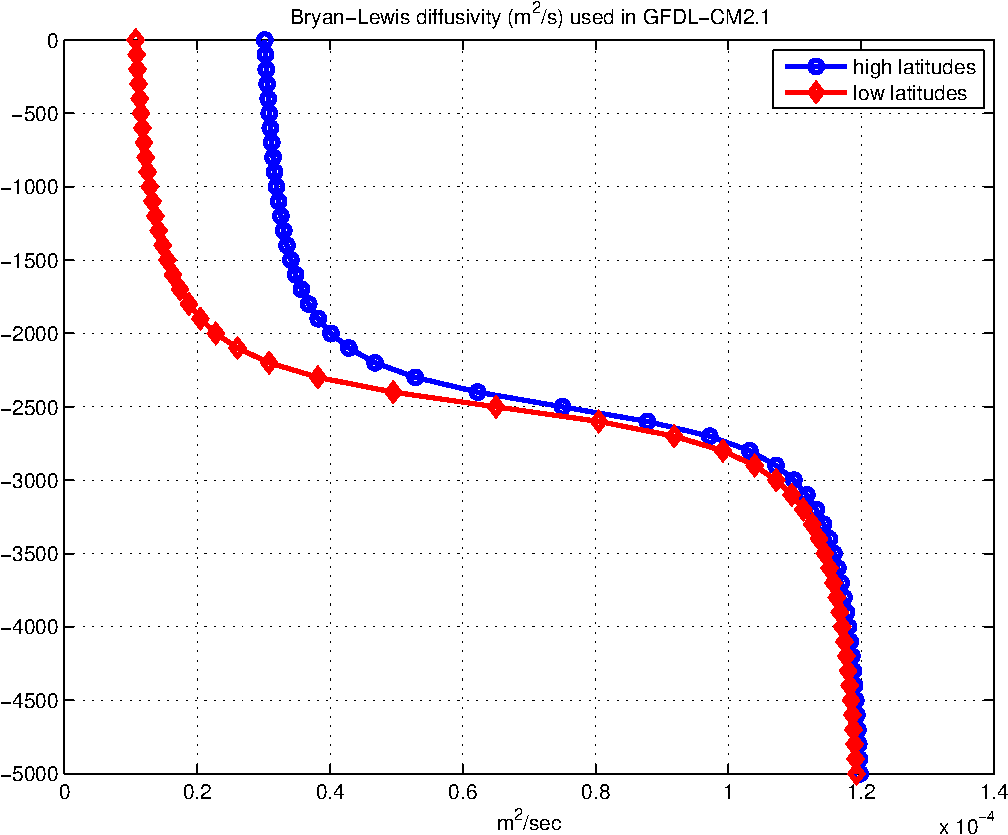
\includegraphics[angle=0,width=8cm]{./figs/bryan_lewis_cm2p1.pdf}
\caption[Bryan-Lewis background diffusivities]{\sf Sample vertical
  profiles for background diffusivities (in units of
  $\mbox{m}^{2}~\mbox{s}^{-1}$) given by the \cite{BryanLewis1979}
  functional form, as used by the OM3 ocean component of the
  GFDL-CM2.1 climate model \citep{OMDT2005a}.  The surface values in
  the tropics are $0.1 \times 10^{-4} \, \mbox{m}^2 \, \mbox{s}^{-1}$,
  whereas they are increased in the high latitudes to $0.3 \times
  10^{-4} \, \mbox{m}^2 \, \mbox{s}^{-1}$.
The Bryan-Lewis coefficients from equation
(\ref{eq:bryan-lewis-function-mom}) for the high latitudes are given
by 
${\tt afkph} =0.75$,
${\tt dfkph} =0.95$,
${\tt sfkph} =4.5 \, \times 10^{-5}$,
${\tt zfkph} =2500$,
and for the equatorial region they are 
${\tt afkph} =0.65$,
${\tt dfkph} =1.15$,
${\tt sfkph} = 4.5 \, \times 10^{-5}$,
${\tt zfkph} =2500$. }
\label{fig:bryan_lewis-profiles}
\end{center}
\rule{\textwidth}{0.005in}
\end{figure}
%%%%%%%%%%%%%%%%%%%%%%%%%%%%%%%%%%%%%%%%%%%%%%%%%%%%%%%%%%%%%%%%%%%%%%%%

The original implementation from \cite{BryanLewis1979} chose the
background as a function only of depth.  However, the CM2.1
implementation shown in Figure \ref{fig:bryan_lewis-lat-depth}
provides an exponential transition from the lower latitude form to the
higher latitude form, with the transition latitude taken as
$35^{\circ}$.  In this way, the background diffusivity is a function
of both latitude and depth.  The resulting diffusivity is shown in
Figure \ref{fig:bryan_lewis-lat-depth}.

%%%%%%%%%%%%%%%%%%%% %%%%%%%%%%%%%%%%%%%%%%%%%
\begin{figure}[h!t]
\rule{\textwidth}{0.005in}
\begin{center}
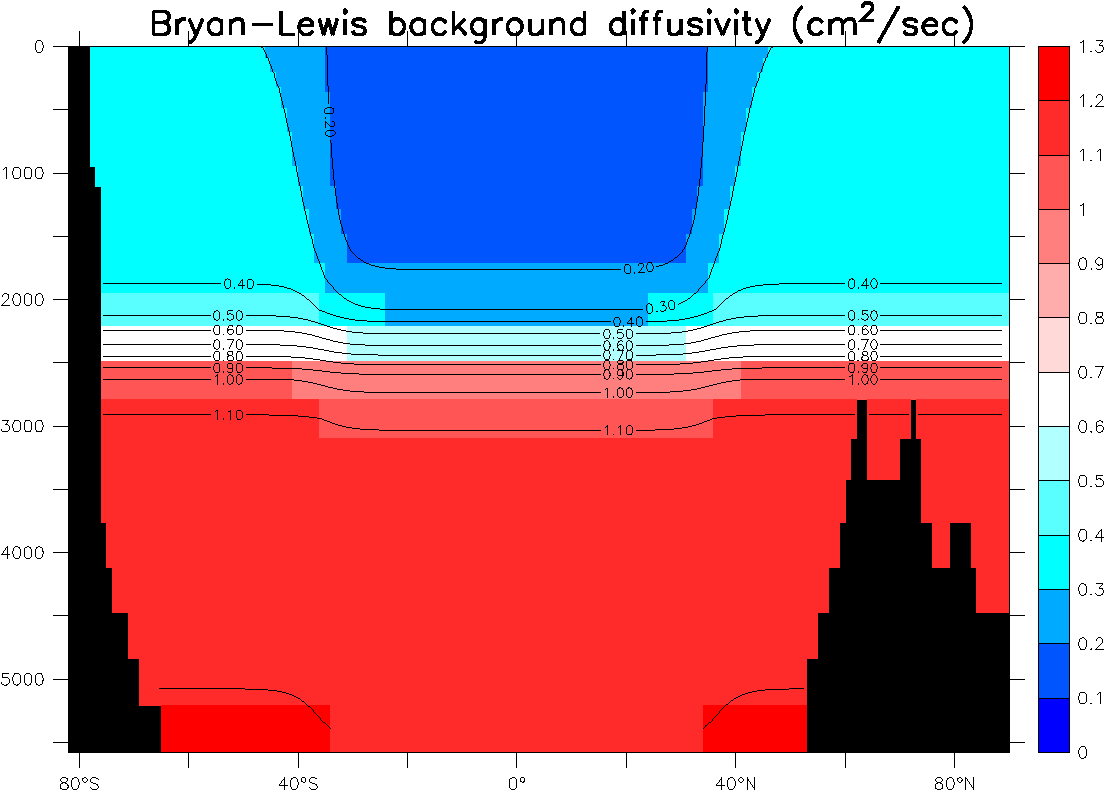
\includegraphics[angle=0,width=8cm]{./figs/bl_diffusivity.pdf}
\caption[Latitude-depth Bryan-Lewis diffusivity]{Shown here is the
  latitude dependent Bryan-Lewis diffusivity
  ($\mbox{cm}^{2}~\mbox{s}^{-1}$) based on values used in GFDL-CM2.1
  configuration discussed in \cite{OMDT2005a}.  The diffusivity is
  composed of the two profiles shown in Figure
  \ref{fig:bryan_lewis-profiles}, with an exponential transition at
  $35^{\circ}$ from the lower values in the tropics to the larger
  values in the high latitudes.}
\label{fig:bryan_lewis-lat-depth}
\end{center}
\rule{\textwidth}{0.005in}
\end{figure}
%%%%%%%%%%%%%%%%%%%%%%%%%%%%%%%%%%%%%%%%%%%%%%%%%%%%%%%%%%%%%%%%%%%%%%%%


\section{The profile from Henyey et al. (1986)} 
\label{section:henyey-diffusivity}

To be completed.  